\chapter{Grundlagen}
\label{chap:grundlagen}

In diesem Kapitel werden zun�chst die grundlegenden
Definitionen und die wichtigsten theoretischen Ergebnisse
der Optimierungstheorie betrachtet.
Wir besch�ftigen uns hier mit Optimierungsproblemen,
die durch differenzierbare Funktionen charakterisiert werden.
Dabei werden verschiedene Optimalit�tsbedingungen von Optimierungsproblemen
gezeigt, die als Grundlage der numerischen Verfahren dienen werden.
Dieses Kapitel orientiert sich an \cite{alt,troeltzsch}.

\section{Allgemeine Optimierungsprobleme}
\begin{definition}
Allgemein ist die Aufgabenstellung der Optimierung wie folgt
definiert:
\begin{equation}
  \min_{x \in \F} f(x) \tag{P} \label{prob:allg_opt_prob}
\end{equation}
Die Funktion $f \colon D \subseteq \R^n \rightarrow \R$ ist die sogennante
Zielfunktion.
$D$ sei der Definitionsbereich von $f$.
$\F$ sei eine nichtleere Teilmenge von $D$, die man als L�sungsmenge bezeichnet.
Alle Elemente von $\F$ werden als zul�ssige Punkte bezeichnet.
$\F$ wird durch die sogennanten Nebenbedingungen oder Restriktionen definiert.
\end{definition}

Falls $\F = D$ gilt,
dann bezeichnet man das Optimierungsproblem als unrestringiert.
Es besitzt also keine Restriktionen.
Ansonsten hei�t es ein restringiertes Optimierungsproblem.

Man definiert in der Regel Optimierungsproblem als ein Minimierungsproblem,
weil ein Maximierungsproblem $\max g(x)$ zu dem Minimierungsproblem
$\min f(x) := -g(x)$ �quivalent ist.

\begin{definition}
\emph{(Globale und lokale L�sung, vgl. Definition 1.1.4 in \cite[S.~2f]{alt})}\\
Ein Punkt $\xopt \in \F$ hei�t globale L�sung des Problems~\eqref{prob:allg_opt_prob} oder
globales Minimum, wenn
\begin{equation}
  f(\xopt) \leq f(x) \qquad \forall x \in \F
\end{equation}
gilt.
Ein Punkt $\xopt \in \F$ hei�t strikte globale L�sung des Problems~\eqref{prob:allg_opt_prob} oder
striktes globales Minimum, wenn
\begin{equation}
  f(\xopt) < f(x) \qquad \forall x \in \F\backslash\{\xopt\}
\end{equation}
gilt.
Ein Punkt $\xopt \in \F$ hei�t lokale L�sung des Problems~\eqref{prob:allg_opt_prob} oder
lokales Minimum, wenn f�r eine Umgebung $U(\xopt)$ von $\xopt$
\begin{equation}
  f(\xopt) \leq f(x) \qquad \forall x \in U(\xopt) \cap \F
\end{equation}
gilt.
Ein Punkt $\xopt \in \F$ hei�t strikte lokale L�sung des Problems~\eqref{prob:allg_opt_prob}
oder striktes lokales Minimum, wenn f�r eine Umgebung $U(\xopt)$ von
$\xopt$
\begin{equation}
  f(\xopt) < f(x) \qquad \forall x \in U(\xopt) \cap \F\backslash\{\xopt\}
\end{equation}
gilt.
Eine Umgebung $U(\xopt)$ von $\xopt$ ist eine offene Menge, die $\xopt$
beinhaltet.
\end{definition}

Wegen dieser Definitionen kommt der Begriff \emph{globale Optimierung}.
Bei der globalen Optimierung versucht man, eine globale L�sung zu finden.
Viele Verfahren versuchen nur lokale L�sungen zu bestimmen,
weil globale L�sungen nicht so einfach zu bestimmen sind.

\begin{example}\label{example:unrestr_opt_prob}
\emph{(vgl. Beispiel 1.1.2 in \cite[S.~1]{alt})}\\
Ein Beispiel eines unrestringierten Optimierungsproblems ist
\begin{equation}
  \min_{x \in \R}\ f(x) := (2x-2)^2 (3x+3)^2 + 10x.
\end{equation}
Dieses Problem hat eine strikte globale L�sung an der Stelle $\xopt = -1$
und eine strikte lokale L�sung an der Stelle $x = 1$
(siehe Abbildung~\ref{fig:beispiel_unrestr_opt_prob}).
\end{example}
\begin{figure}[ht]
\centering
\begin{tikzpicture}[yscale=0.7,xscale=2.5]
  \draw[very thin,color=gray,ystep=2,xstep=0.5] (-1.47,-2.9) grid (1.47,7.4);
  \draw[->] (-1.48,0) -- (1.48,0) node [above] {$x$};
  \draw[->] (0,-3) -- (0,7.5) node [right] {$f(x)$};
  \foreach \x/\xtext in {-1,-0.5/-\frac{1}{2},0,0.5/\frac{1}{2},1}
    \draw (\x,0.1) -- (\x,-0.1) node [below,fill=white] {$\xtext$};
  \foreach \y/\ytext in {-2/-20,0,2/20,4/40,6/60}
    \draw (0.03,\y) -- (-0.03,\y) node [left,fill=white] {$\ytext$};
  \draw[color=blue] plot[smooth] file {images/beispiel-unrestr-opt-prob.table};
\end{tikzpicture}
\caption{Die Funktion von Beispiel \ref{example:unrestr_opt_prob}}
\label{fig:beispiel_unrestr_opt_prob}
\end{figure}

\begin{definition}
\emph{(Nichtlineare Optimierungsprobleme)}
Die Aufgabenstellung bei der nichtlinearen Optimierung
mit Gleichungs- und Ungleichungsrestriktionen kann man
spezifischer wie folgt definieren:
\begin{align}
  \min_{x \in D}\ & f(x) \tag{PN}\label{prob:opt_prob_mit_nichtlin_restr} \\
              \nb & g(x) \leq 0 \notag \\
                  & h(x) = 0 \notag
\end{align}
Die Zielfunktion ist wieder die Funktion
$f \colon D \subseteq \R^n \rightarrow \R$.
Die Nebenbedingungen sind von den Funktionen
$g \colon D \subseteq \R^n \rightarrow \R^p$ und
$h \colon D \subseteq \R^n \rightarrow \R^m$ abh�ngig.
D.\,h., die Menge $\F$ sieht hier so aus:
$\F = \{ x \in \R^n \,|\, g(x) \leq 0, \, h(x) = 0  \}$.
\end{definition}

Die Bezeichnung ``Nb.'' steht hier als Abk�rzung f�r
``unter der Nebenbedingung'' oder ``unter den Nebenbedingungen''.
Die Operatoren $\leq$ und $=$ vergleichen hier die Vektoren
miteinander elementenweise.
Die Zahl $0$ hier
ist je nach dem in welchem Kontext
ein Element von $\R$, $\R^p$ oder $\R^m$.

Man kann das Problem~\ref{prob:opt_prob_mit_nichtlin_restr}
ausf�hrlicher schreiben, indem man die Funktionen
$g$ und $h$ in skalare Funktionen $g_1, \ldots, g_p \colon \R^n \rightarrow \R$
und $h_1, \ldots, h_m \colon \R^n \rightarrow \R$ zerlegt, so dass
\begin{equation*}
  g(x) =
    \left(
    \begin{array}{c}
      g_1(x) \\
      \vdots \\
      g_p(x)
    \end{array}
    \right)
\quad \text{und} \quad
  h(x) =
    \left(
    \begin{array}{c}
      h_1(x) \\
      \vdots \\
      h_m(x)
    \end{array}
    \right).
\end{equation*}

Man bekommt dann das Problem
\begin{align*}
  \min_{x \in D}\ & f(x) \\
              \nb & g_i(x) \leq 0 \text{ f�r } i = 1,\ldots,p \\
                  & h_j(x) = 0 \text{ f�r } j = 1,\ldots,m.
\end{align*}

Man kann hierbei den Unterschied zwischen der linearen Optimierung und
der nichtlinearen Optimierung gut erkennen.
Bei der linearen Optimierung muss die Zielfunktion linear sein
(d.\,h., die Zielfunktion muss in der Form $f(x) = c^T x$, $c \in \R^n$, sein)
und die Nebenbedingungen sollen durch lineare Gleichungen bzw.
Ungleichungen definiert werden.
Bei der nichtlinearen Optimierung gibt es dagegen keine Einschr�nkung,
wie die Zielfunktion und die Nebenbedingungen aussehen sollen.

\begin{example}\label{example:opt_prob_mit_nichtlin_restr}
\emph{(vgl. Problem 1.2 in \cite[S.~3]{nocedal})}\\
Ein Beispiel eines restringierten Optimierungsproblems ist
\begin{equation}
\begin{split}
  \min_{x \in \R^2}\ (x_1-2)^2 & + (x_2-1)^2 \\
  \nb x_1 + x_2 & \leq 2 \\
          x_1^2 & \leq x_2.
\end{split}
\end{equation}
Die Abbildung~\ref{fig:beispiel_opt_prob_mit_nichtlin_restr}
zeigt die zul�ssige Menge $\F$,
die H�henlinien der Zielfunktion und
die optimale L�sung~$\xopt$.
\end{example}
Die H�henlinie ist eine Menge von Punkten,
wo die Zielfunktion einen konstanten Wert nimmt.
In der Abbildung~\ref{fig:beispiel_opt_prob_mit_nichtlin_restr}
sind die H�henlinien in Form von Kreisen zu sehen
und je gr��er der Kreis ist,
desto gr��er ist der Wert der Zielfunktion.
\begin{figure}[h]
\centering
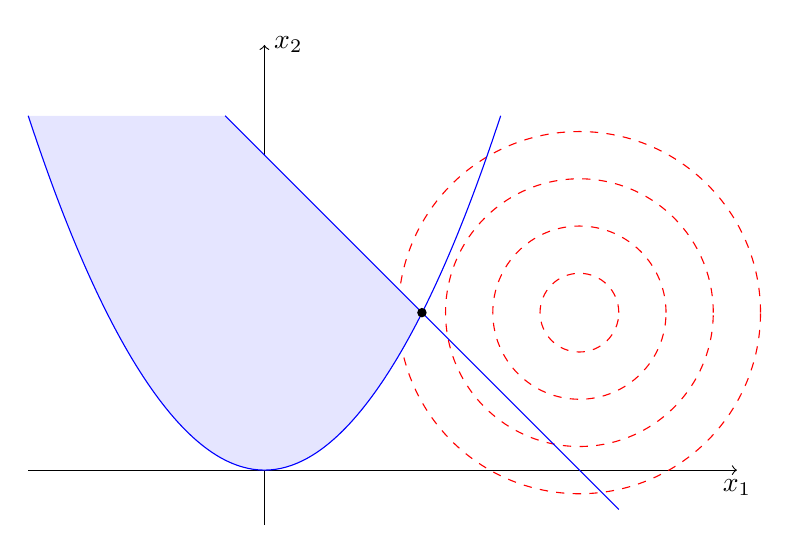
\begin{tikzpicture}[scale=2]
  \draw[->] (-1.5,0) -- (3,0) node [below] {$x_1$};
  \draw[->] (0,-0.35) -- (0,2.7) node [right] {$x_2$};
  % Die H�henlinien
  \foreach \r in {0.25, 0.55, 0.85, 1.15}
    \draw[dashed,color=red] (2,1) circle (\r);
  % Schreibe x*
  \draw (1.02,1.05) node[right,fill=white] {$\xopt$};
  % Die zul�ssige Menge F
  \fill[blue!10] (0,0) parabola (-1.5,2.25)
    (0,0) parabola (1,1) -- (-0.25,2.25) -- (-1.5,2.25);
  \draw (0,1) node {$\F$};
  % Die Nebenbedingungen
  \draw[color=blue] (0,0) parabola (-1.5,2.25) (0,0) parabola (1.5,2.25);
  \draw[color=blue] (-0.25,2.25) -- (2.25,-0.25);
  % Der Kreis f�r x*
  \fill (1,1) circle (0.03);
\end{tikzpicture}
\caption{Geometrische Darstellung
des Beispiels~\ref{example:opt_prob_mit_nichtlin_restr}}
\label{fig:beispiel_opt_prob_mit_nichtlin_restr}
\end{figure}

\section{Optimierungsprobleme ohne Restriktionen}
Wir beginnen nun zuerst mit Optimierungsproblemen ohne Restriktionen
und stellen die notwendigen und hinreichenden Optimalit�tsbedingungen bereit.
Zwei numerische Verfahren hierf�r werden auch vorgestellt.

\begin{definition}
\emph{(Unrestringierte Optimierungsprobleme)}
\begin{equation}
  \min_{x \in \R^n} f(x). \tag{PU} \label{prob:opt_prob_unrestr}
\end{equation}
Wir nehmen hier der Einfachheit halber an, dass der Definitionsbereich
$D$ gleich $\R^n$ sei.
\end{definition}

\begin{example}\label{example:lineare_regression}
\emph{(Lineare Regression, vgl. Beispiel 1.1.6 in \cite[S.~4~f.]{alt})}\\
Ein praktisches Beispiel ist
die Aufgabe der linearen Regression.
Gegeben seien m Messwerte
$(\xi_1,\eta_1),\ldots,(\xi_m,\eta_m)$.
Gesucht ist eine Gerade
\begin{equation}
  \eta(\xi) := x_1 \xi + x_2,
\end{equation}
die \textss{optimal} zu den Messwerten passt.
D.\,h., der Parameter $x = (x_1,x_2)^T \in \R^2$
soll so bestimmt werden, dass die Summe der Fehlerquadrate
in den Messpunkten minimiert wird.
Somit ist ein unrestringiertes Optimierungsproblem
\begin{equation}
  \min_{x \in \R^2}\ 
  f(x) := \sum_{i=1}^{m} (\eta(\xi_i) - \eta_i)^2
        = \sum_{i=1}^{m} (x_1 \xi_i + x_2 - \eta_i)^2
\end{equation}
zu l�sen.
\end{example}

\begin{example}\label{example:nichtlineare_regression}
\emph{(Nichtlineare Regression, vgl. Abschnitt 2.3.2 in \cite[S.~30~f.]{alt})}\\
Neben linearen Regressionsaufgaben sind auch oft
nichtlineare Regressionsaufgaben zu l�sen.
Gesucht ist der funktionale Zusammenhang $\eta(\xi)$
zwischen den $\xi$- und den $\eta$-Werten,
beispielsweise
\begin{equation}\label{eq:nichtlin_regres_quad_zusammenhang}
  \eta(\xi) := x_1 (\xi -x_2)^2 + x_3
\end{equation}
oder
\begin{equation}\label{eq:nichtlin_regres_exp_zusammenhang}
  \eta(\xi) := x_1 e^{\xi x_2}.
\end{equation}
Dabei ist $x = (x_1,\ldots,x_n)^T \in \R^n$ ein Parametervektor,
der \textss{optimal}
bestimmt werden soll.
\end{example}

\begin{theorem}
\label{satz:notw_bed_fuer_unrestr_prob}
\emph{(Notwendige Bedingung erster Ordnung, vgl. Satz 3.1.2 in
\cite[S.~42]{alt})}\\
Sei $\xopt$ eine lokale L�sung des Problems~(\ref{prob:opt_prob_unrestr}) und
sei $f$ einmal stetig differenzierbar in einer Umgebung von $\xopt$,
dann gilt
\begin{equation}
  \nabla f(\xopt) = 0. \label{eq:grad_zero}
\end{equation}
\end{theorem}

Die Bedingung~\eqref{eq:grad_zero} gilt aber nicht nur f�r lokale Minima
sondern auch f�r lokale Maxima von~$f$.

\begin{definition}
\emph{(Station�rer Punkt, vgl. Definition 3.1.4 in \cite[S.~42]{alt})}\\
Die Funktion $f$ sei in $\xopt$ differenzierbar. Der Punkt $\xopt$ hei�t
station�rer Punkt von $f$, wenn $\xopt$ die notwendige Bedingung~(\ref{eq:grad_zero})
erf�llt.
\end{definition}

Viele Optimierungsverfahren suchen in der Regel nach einem station�ren Punkt
von~$f$.
Aber ein station�rer Punkt muss kein globales oder lokales Minimum sein.
Durch folgende notwendige Bedingung kann man zwischen einem lokalen Minimum und
einem lokalen Maximum unterscheiden.

\begin{theorem}
\emph{(Notwendige Bedingung zweiter Ordnung, vgl. Satz 3.1.6 in
\cite[S.~43]{alt})}\\
Sei $\xopt$ eine lokale L�sung des Problems~(\ref{prob:opt_prob_unrestr})
und sei $f$ zweimal stetig differenzierbar in einer Umgebung von $\xopt$,
dann gilt~(\ref{eq:grad_zero}) und
\begin{equation}
  x^T f''(\xopt) x \geq 0 \qquad \forall x \in \R^n.
\end{equation}
$f''(\xopt)$ ist also positiv semidefinit.
\end{theorem}

\begin{theorem}
\emph{(Hinreichende Bedingung zweiter Ordnung, vgl. Satz 3.1.11 in
\cite[S.~44]{alt})}\\
Sei $f$ zweimal stetig differenzierbar in einer Umgebung von $\xopt$.
Die notwendige Bedingung~(\ref{eq:grad_zero}) sei erf�llt und $f''(\xopt)$
sei positiv definit, d.\,h.
\begin{equation}
  x^T f''(\xopt) x > 0 \qquad \forall x \in \R^n.
\end{equation}
Dann ist $\xopt$ eine strikte L�sung des Problems~(\ref{prob:opt_prob_unrestr}).
\end{theorem}

Diese hinreichende Bedingung benutzt man in der Regel erst dann, wenn man einen
station�ren Punkt findet.

Eine wichtige Grundlage f�r einige Verfahren ist
die Definition der Abstiegsrichtung.

\begin{definition}
\label{def:abstiegsrichtung}
\emph{(Abstiegsrichtung, vgl. Definition 4.1.2 in \cite[S.~68]{alt})}\\
Die Funktion $f$ sei differenzierbar in $x$. Ein Vektor
$d \in \R^n\backslash\{0\}$ hei�t Abstiegsrichtung von~$f$ in~$x$, wenn
\begin{equation}
  \nabla f(x)^T d < 0
\end{equation}
gilt.
\end{definition}

Sei $x \in \R^n$ mit $\nabla f(x) \neq 0$, dann ist beispielsweise $d = - \nabla
f(x)$ eine Abstiegsrichtung von~$f$ in~$x$.

\begin{theorem}
\label{satz:existenz_von_schrittweite}
\emph{(Vgl. Lemma 4.1.1 in \cite[S.~68]{alt})}\\
Seien $x \in \R^n$, $f$ differenzierbar in $x$ und $d$
eine Abstiegsrichtung von $f$ in $x$. Dann gibt es ein $\hat{\sigma} > 0$ mit
\begin{equation}
  f( x + \sigma d) < f(x) \qquad \forall \sigma \in \ ]0, \hat{\sigma}[.
\end{equation}
\end{theorem}

Die meisten Optimierungsverfahren sind iterativ. Sie fangen also mit einem
Anfangspunkt $x^0$ an und versuchen dann weitere Punkte ($x^1, x^2, \ldots , x^k
, \ldots$) zu finden, die besser als die vorherigen sind.
Viele iterative Verfahren zur Bestimmung einer lokalen L�sung sind h�ufig
Abstiegsverfahren. In der $k$-ten Iteration bestimmen sie zu einem Punkt~$x^k$
eine Abstiegsrichtung~$d^k$ und eine Schrittweite $\sigma_k$ so, dass f�r
$x^{k+1} := x^k + \sigma_k d^k$
\begin{equation}
  f(x^{k+1}) < f(x^k)
\end{equation}
gilt.

\subsection{Gradientenverfahren}

Das Gradientenverfahren ist ein einfaches Abstiegsverfahren,
welches die negativen Gradienten als Abstiegsrichtungen verwendet.

\begin{algorithm}
\emph{(Gradientenverfahren, vgl. Verfahren 4.2.39 in \cite[S.~98]{alt})}
\begin{enumerate}
  \item W�hle einen Startpunkt $x^0$ und setze $k := 0$.
  \item Setze $d^k := - \nabla f(x^k)$. \label{list:compute_d_in_grad_verf}
  \item Ist $d^k = 0$ $\Rightarrow$ STOP. \label{list:stop_criteria_grad_verf}
  \item Bestimme Schrittweite $\sigma_k$ so, dass
        \begin{equation}
          f(x^k + \sigma_k d^k) < f(x^k + \sigma d^k)
            \qquad \forall \sigma \geq 0.
        \end{equation}
  \item Setze $x^{k+1} := x^k + \sigma_k d^k$ und $k := k+1$. $\Rightarrow$
        Gehe zu Schritt~\ref{list:compute_d_in_grad_verf}.
\end{enumerate}
\end{algorithm}

Es ist zu beachten, dass die Abbruchbedingung in
Schritt~\ref{list:stop_criteria_grad_verf}
nur theoretisch zu verstehen ist.
Praktisch gibt man eine Abbruchschranke $\varepsilon > 0$ vor
und f�hrt beispielsweise den Test
\begin{equation}
  \|d^k\| < \varepsilon
\end{equation}
durch.

Zur Bestimmung der Schrittweite $\sigma_k$ kann man das
Schrittweitenverfahren von Armijo oder das Schrittweitenverfahren von
Wolfe-Powell verwenden (vgl. Abschnitt 4.2.7 in \cite[S.~90~ff.]{alt}).

\subsection{Newton-Verfahren} \label{sec:newton_verfahren}

Ein bekanntes Verfahren der numerischen Mathematik, um eine nichtlineare
Gleichung zu l�sen, ist das Newton-Verfahren.
Man berechnet mit dem Newton-Verfahren eine Nullstelle
von einer gegebenen Abbildung $F:\R^n \rightarrow \R^n$,
d.\,h. eine L�sung $\xopt \in \R^n$ der nichtlinearen Gleichung $F(x) = 0$.
F�r die unrestringierten Optimierungsprobleme kann das Newton-Verfahren
angewendet werden, um die L�sung der nichtlinearen
Gleichung~\eqref{eq:grad_zero},
$\nabla f(x) = 0$, zu finden.
Es wird dabei vorausgesetzt,
dass die Funktion $f$ zweimal differenzierbar ist.

\begin{algorithm}
\emph{(Newton-Verfahren, vgl. Verfahren 4.3.1 in \cite[S.~107]{alt})}
\begin{enumerate}
  \item W�hle einen Startpunkt $x^0$ und setze $k := 0$.
  \item Ist $\nabla f(x^k) = 0$ \label{list:stop_criteria_newt_verf}
        $\Rightarrow$ STOP.
  \item Berechne die L�sung $d$ des linearen Gleichungssystems
        \begin{equation}
          f''(x^k) d = - \nabla f(x^k).
        \end{equation}
        Setze $d^k := d$.
  \item Setze $x^{k+1} := x^k + d^k$ und $k := k+1$ $\Rightarrow$
        Gehe zu Schritt~\ref{list:stop_criteria_newt_verf}.
\end{enumerate}
\end{algorithm}

Der Punkt $x^{k+1}$ in jedem Iterationsschritt ist eigentlich die L�sung des
Minimierungsproblems, welches durch die quadratische Approximation von $f$ in Punkt $x^k$ definiert ist.
In der Umgebung von $x^k$ kann die Funktion $f$ wie folgt approximiert werden:
\begin{equation}
  f(x) \approx f(x^k) + \nabla f(x^k)^T (x-x^k)
                 + \frac{1}{2} (x-x^k)^T f''(x^k) (x-x^k).
\end{equation}
Die Ableitung der rechten Seite ist
\begin{equation}
  \nabla f(x^k) + f''(x^k) x - f''(x^k) x^k.
\end{equation}
Setzt man diese gleich null, dann bekommt man
\begin{align}
  f''(x^k) (x-x^k) & = - \nabla f(x^k) \\
            x-x^k  & = - [f''(x^k)]^{-1} \nabla f(x^k) \\
            x      & = x^k \underbrace{- [f''(x^k)]^{-1} \nabla f(x^k)}_{d}.
\end{align}
Das ist genau unser Punkt $x^{k+1}$.
D.\,h., es wird in jedem Iterationsschritt eigentlich das Problem
\begin{equation}
  \min_{x \in \R^n}\ f(x^k) + \nabla f(x^k)^T (x-x^k)
                 + \frac{1}{2} (x-x^k)^T f''(x^k) (x-x^k)
\end{equation}
gel�st, wobei die Konstante $f(x^k)$ weggelassen werden kann.

Es ist sp�ter zu sehen, dass das SQP-Verfahren diese Idee auch
gebrauchen wird.

Eine Schrittweitensteuerung wie bei dem Gradientenverfahren kann auch
durchgef�hrt werden, d.\,h., man bestimmt ein $\sigma_k \in \R$ und definiert
$x^{k+1} := x^k + \sigma_k d^k$.
Dann bekommt man ein Abstiegsverfahren,
welches als das ged�mpfte Newton-Verfahren bezeichnet wird
(vgl. Abschnitt 4.3.2 in \cite[S.~111~ff.]{alt}).

\section{Optimierungsprobleme mit linearen Restriktionen}

  Nun ist die Theorie der restringierten Optimierungsprobleme
  zu betrachten.
  Wir konzentrieren uns vorerst auf lineare Restriktionen,
  d.\,h., die Nebenbedingungen sind durch lineare Gleichungen und Ungleichungen
  definiert.

  \subsection{Optimierungsprobleme mit linearen Gleichungsnebenbedingungen}
  \begin{definition}
\emph{(Optimierungsproblem mit linearen Gleichungsnebenbedingungen)}
\begin{align}
  \min_{x \in \R^n}\ & f(x) \tag{PLG}\label{prob:opt_prob_mit_lin_gl_nebenbed}\\
              \nb & Ax = b \notag
\end{align}
$A$ sei eine $(m \times n)$-Matrix und $b$ sei ein Vektor mit $m$ Elementen.
\end{definition}

D.\,h., die Menge $\F$ sieht hier so aus:  $\F = \{ x \in \R^n\ |\ A x = b \}$.

\begin{theorem}
\emph{(Notwendige Bedingung erster Ordnung)}
Sei $\xopt$ eine lokale L�sung des
Problems~\eqref{prob:opt_prob_mit_lin_gl_nebenbed}
und $f$ sein in $\xopt$ differenzierbar.
Dann gibt es ein $\lambda \in \R^m$ mit
\begin{equation}
  \nabla f(\xopt) + A^T \lambda = 0.
\end{equation}
Hat A einen vollen Rang, dann ist $\lambda$ eindeutig zu bestimmen.
\end{theorem}

Diese Bedingung hei�t die Multiplikatoren Regel von Lagrange. Man bezeichnet
$\lambda$ als die Lagrange-Multiplikator.

\begin{theorem}
\emph{(Hinreichende Bedingung zweiter Ordnung)}
Sei $f$ in $\xopt$ zweimal stetig differenzierbar. Die notwendige Bedingung
erster Ordnung sei erf�llt. Es g�be eine Konstante $\alpha > 0$ mit
\begin{equation}
  d^T f''(x) d \geq \alpha \|d\|^2 \qquad \forall d \in \kr A.
\end{equation}
Dann ist $\xopt$ eine strikte L�sung des linearen restringierten Problems.
\end{theorem}

\begin{definition}%TODO Einleitung schreiben ..
\emph{(Nullraum-Matrix)}
Eine $(n \times l)$-Matrix $Z$ hei�t Nullraum-Matrix von~$A$, wenn f�r $d \in
\R^n$ gilt
\begin{equation}
d \in \kr A \quad \Leftrightarrow \quad d = Z z \text{ f�r ein } z \in \R^l.
\end{equation}
D.\,h. $\im Z = \kr A$.
\end{definition}

Sei $w$ eine L�sung von der Gleichung $Ax=b$. Man kann nun f�r $\F$ so
schreiben:
\begin{equation}
  \F = w + \kr A = w + \im Z = w + \{ Z z | z \in \R^l \}.
\end{equation}

Das Problem~\eqref{prob:opt_prob_mit_lin_gl_nebenbed} ist dann �quivalent zu
\begin{equation}
  \min_{z \in \R^l} F(z) := f(w + Zz).
\end{equation}
Dieses Problem hat keine Nebenbedingung mehr, also unrestringiert.
Man kann also die Verfahren f�r unrestringierte Probleme anwenden.
Wir werden aber nachher sehen, wie man dieses Problem effektiv l�sen kann,
wenn die Zeilfunktion quadratisch ist.

  \subsection{Optimierungsprobleme mit linearen Ungleichungsnebenbedingungen}
  \begin{definition}
\emph{(Optimierungsprobleme mit linearen Ungleichungsnebenbedingungen)}
\begin{align}
  \min_{x \in \R^n}\ & f(x)
    \tag{PLU} \label{prob:opt_prob_mit_lin_ungl_nebenbed} \\
                 \nb & Ax = b \notag \\
                     & Gx \leq r \notag
\end{align}
$A$ sei eine $(m \times n)$-Matrix mit $m \leq n$ und $b \in \R^m$.
$G$ sei eine $(p \times n)$-Matrix und $r \in \R^p$.
\end{definition}

D.\,h., die Menge $\F$ sieht hier so aus:
$\F = \{ x \in \R^n\ |\ A x = b,\ G x \leq r \}$.

Seien $a_k \in \R^n$, $k = 1,\ldots,m$, bzw. $g_j \in \R^n$, $j = 1,\ldots,p$,
Vektoren in der Matrix $A$ bzw. $G$, so dass
\begin{equation}
  A =
  \left(
    \begin{array}{c}
      a_1^T \\
      \vdots \\
      a_m^T
    \end{array}
  \right)
\quad \text{und} \quad
  G =
  \left(
    \begin{array}{c}
      g_1^T \\
      \vdots \\
      g_p^T
    \end{array}
  \right).
\end{equation}

Seien $b_k \in \R$, $k = 1,\ldots,m$, bzw. $r_j \in \R$, $j = 1,\ldots,p$,
die Elemente von $b$ bzw. $r$.
Dann k�nnen wir das Problem~\eqref{prob:opt_prob_mit_lin_ungl_nebenbed}
wie folgt ausf�hrlicher schreiben.
\begin{align*}
  \min_{x \in \R^n}\ & f(x) \\
     \nb & \langle a_k, x \rangle = b_k \text{ f�r } k = 1,\ldots,m \\
         & \langle g_j, x \rangle \leq r_j \text{ f�r } j = 1,\ldots,p
\end{align*}

\begin{example}\label{example:abstand_zw_dreiecken_problem}
Gegeben seien zwei Dreiecke $R$ und $S$
in der Abbildung~\ref{fig:abstand_zw_dreiecken}.
Gesucht ist der k�rzeste Abstand zwischen diesen Dreiecken
und die zugeh�rigen Punkte $r^* \in R$ und $s^* \in S$, die
diesen k�rzesten Abstand bilden.
\end{example}

Seien $r = (x_1, x_2)^T \in R$ und $s = (x_3, x_4)^T \in S$.
Der quadratische Abstand zwischen $r$ und $s$ ist durch
\begin{equation}
  \| r - s \|^2 = (x_1 - x_3)^2 + (x_2 - x_4)^2 = x^T H x
\end{equation}
gegeben, wobei
\begin{equation}
  H :=
  \left(\begin{array}{cccc}
     1 &  0 & -1 &  0 \\
     0 &  1 &  0 & -1 \\
    -1 &  0 &  1 &  0 \\
     0 & -1 &  0 &  1
  \end{array}\right).
\end{equation}

Die Bedingungen $r \in R$ und $s \in S$ sind durch die Ungleichungen
\begin{equation}
\begin{split}
    x_1, x_2 & \geq 0 \\
  x_1 + 2x_2 & \leq 2 \\
         x_4 & \geq 2 \\
   x_3 + x_4 & \geq 3 \\
  x_3 + 2x_4 & \leq 6
\end{split}
\end{equation}
gegeben.
D.\,h. das Problem kann als ein Optimierungsproblem mit einer quadratischen
Zielfunktion und linearen Ungleichungsnebenbedingungen dargestellt werden.

\begin{figure}[h]
\centering
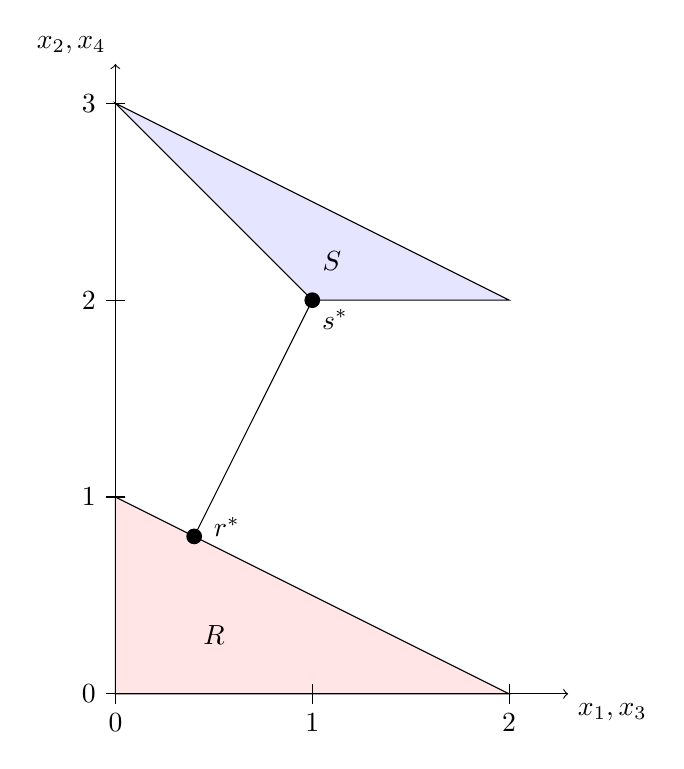
\begin{tikzpicture}[scale=2.5]
  % Dreieck R
  \draw[fill=red!10] (0,0) -- (0,1) -- (2,0) -- cycle;
  \draw (0.5,0.3) node {$R$};
  % Dreieck S
  \draw[fill=blue!10] (0,3) -- (1,2) -- (2,2) -- cycle;
  \draw (1.1,2.2) node {$S$};
  % Punkt r*
  \fill (0.4,0.8) circle (0.04);
  \draw (0.45,0.85) node [right] {$r^*$};
  % Punkt s*
  \fill (1,2) circle (0.04);
  \draw (1,2) node [below right] {$s^*$};
  % Linie zwischen r* und s*
  \draw (0.4,0.8) -- (1,2);
  % Koordinatenachsen
  \draw[->] (0,0) -- (2.3,0) node [below right] {$x_1, x_3$};
  \foreach \x in {0,...,2}
    \draw (\x,0.05) -- (\x,-0.05) node [below] {\x};
  \draw[->] (0,0) -- (0,3.2) node [above left] {$x_2, x_4$};
  \foreach \y in {0,...,3}
    \draw (0.05,\y) -- (-0.05,\y) node [left] {\y};
\end{tikzpicture}
\caption{Geometrische Darstellung
des Beispiels~\ref{example:abstand_zw_dreiecken_problem}}
\label{fig:abstand_zw_dreiecken}
\end{figure}

Der folgende Satz hat sich als besonders hilfreich erwiesen,
um eine lokale L�sung
des Problems~\eqref{prob:opt_prob_mit_lin_ungl_nebenbed}
zu charakterisieren.

\begin{theorem} \label{satz:karush_kuhn_tucker}
\emph{(Karush-Kuhn-Tucker-Satz, vgl. Satz 5.4.7 in \cite[S.193]{alt})}\\
Sei $\xopt$ lokale L�sung des Problems~\eqref{prob:opt_prob_mit_lin_ungl_nebenbed} und
$f$ sei in~$\xopt$ differenzierbar.
Dann existieren die Vektoren $\lambda \in \R^m$ und $\mu \in \R^p$
zu~$\xopt$ mit
\begin{align}
   \nabla f(\xopt) + A^T \lambda + G^T \mu & = 0 \\
  \mu_j (\langle g_j,\xopt \rangle - r_j ) & = 0 \text{ f�r } j = 1,\ldots,p \\
                                       \mu & \geq 0
\end{align}
Die Vektoren $\lambda$ und $\mu$ hei�en Lagrange-Multiplikatoren zu $\xopt$.
\end{theorem}

Sei $x \in \F$. Wir bezeichnen mit
\begin{equation}
  J(x) := \{ 1 \leq j \leq p \ | \ \langle g_j,x \rangle = r_j \}
\end{equation}
die Indexmenge der in $x$ aktiven Ungleichungsrestriktionen.

\begin{theorem}
\emph{(Hinreichende Optimalit�tsbedingung, vgl. Satz 5.4.13 in
\cite[S.~198]{alt})}\\
Sei $f$ in $\xopt \in \F$ zweimal stetig differenzierbar. Die notwendigen
Bedingungen von Satz~\ref{satz:karush_kuhn_tucker} seien erf�llt
und es gelte mit $\alpha > 0$
\begin{equation}
d^T f''(\xopt) d \geq \alpha \|d\|^2 \quad
  \forall d \in \R^n :
  \begin{cases}
    Ad = 0, & \\
    \langle g_j,d \rangle \leq 0
      & \text{f�r } j \in J(\xopt) \text{ mit } \mu_j = 0, \\
    \langle g_j,d \rangle = 0
      & \text{f�r } j \in J(\xopt) \text{ mit } \mu_j > 0.
  \end{cases}
\end{equation}
Dann ist $\xopt$ eine strikte lokale L�sung des
Problems~\eqref{prob:opt_prob_mit_lin_ungl_nebenbed}.
\end{theorem}

Ein Spezialfall des Problems~\eqref{prob:opt_prob_mit_lin_ungl_nebenbed} ist das
Optimierungsproblem mit unteren und oberen Schranken f�r die Variablen.

\begin{definition}
\emph{(Optimierungsprobleme mit Variablenbeschr�nkungen)}
\begin{align}
  \min_{x \in \R^n}\ & f(x) \tag{PVB} \label{prob:opt_prob_mit_var_beschr} \\
                 \nb & a \leq x \leq b \notag
\end{align}
$a, b \in \R^n$ mit $a \leq b$.
\end{definition}

Die Nebenbedingung ist
�quivalent zu
$G x \leq r$
mit
$G := \left( \begin{array}{c} -I_n \\ I_n \end{array} \right)$ und
$r := \left( \begin{array}{c} -a \\ b \end{array} \right)$.

% TODO: sufficient condition?


\section{Optimierungsprobleme mit nichtlinearen Restriktionen}
Wir kommen nun zu dem allgemeinen nichtlinearen Optimierungsproblem.
Wir schreiben noch einmal das Problem~\eqref{prob:opt_prob_mit_nichtlin_restr}.
\begin{align*}
  \min_{x \in \R^n}\ & f(x) \\
              \nb & g_i(x) \leq 0 \text{ f�r } i = 1,\ldots,p \\
                  & h_j(x) = 0 \text{ f�r } j = 1,\ldots,m
\end{align*}

Um die Optimalit�tsbedingung des Problems~\eqref{prob:opt_prob_mit_nichtlin_restr}
zu bekommen, definiert man die sogenannte Regularit�tsbedingung
(vgl. Definition 7.2.14 in \cite[S.~261]{alt}),
die wir hier nicht n�her betrachten werden.
Die folgende Definition ist eine spezielle Bedingung,
aus der diese Regularit�tsbedingung folgt.
Diese Regularit�tsbedingung kann aber
noch von anderen Bedingungen hergeleitet werden.

\begin{definition}
\emph{(Mangasarian-Fromowitz-Regularit�tsbedingung, vgl. Satz 7.2.24 in
\cite[S.~270]{alt})}
Sei $x \in \F$. Mit
$\,\I(x) := \{ i \in \{1,\ldots,p\} \ | \ g_i(x) = 0 \}$
wird die Indexmenge der in $x$ aktiven Ungleichungsrestriktionen bezeichnet.
Seien $g_i$ und $h_j$ differenzierbar in~$x$
f�r $i=1,\ldots,p$ und $j=1,\ldots,m$.
Der Punkt $x$ erf�llt die Mangasarian-Fromowitz-Regularit�tsbedingung,
wenn die Gradienten
\begin{equation}
 \nabla h_j(x),\ j = 1,\ldots,m, \text{ linear unabh�ngig}
\end{equation}
sind und ein Vektor $d \in \R^n$ mit
\begin{equation}
  \nabla g_i(x)^T d < 0,\ i \in \I(x)
  \quad \text{und} \quad
  \nabla h_j(x)^T d = 0,\ j = 1,\ldots,m
\end{equation}
existiert.
\end{definition}

Der folgende Satz gilt eigentlich mit der allgemeinen Regularit�tsbedingung.
Wir verwenden aber hier nur die Mangasarian-Fromowitz-Regularit�tsbedingung.

\begin{theorem}
\emph{(Notwendige Bedingung, vgl. Satz 7.2.11 in \cite[S.~260]{alt})}\\
Sei $\xopt$ eine lokale L�sung des
Problems~\eqref{prob:opt_prob_mit_nichtlin_restr} und $\xopt$ erf�lle die
Mangasarian-Fromowitz-Regularit�tsbedingung.
Sei $f$ in $\xopt$ differenzierbar.
Dann existieren Vektoren $\lambda \in \R^m$ und $\mu \in \R^p$,
sodass
\begin{gather}
  \nabla f(\xopt) + \sum_{i=1}^{m} \lambda_i \nabla h_i(\xopt)
    + \sum_{j=1}^{p} \mu_j \nabla g_j(\xopt) = 0 \\
  \mu_j \geq 0, \quad \mu_j g_j(\xopt) = 0, \quad
  j=1,\ldots,p
\end{gather}
\end{theorem}

F�r die hinreichende Bedingung zweiter Ordnung verweisen wir auf Satz 7.3.1
in \cite[S.~273]{alt}.

% TODO: Approximation der Gradient und Hesse-Matrix?
